% Richard James Howe
% LaTeX Final Year Project, final report.
% Fri Apr 19 23:17:27 BST 2013
\documentclass	[a4paper, 10pt]	{article}
\usepackage	    [T1]		        {fontenc}
\usepackage	    [utf8]		      {inputenc}
\usepackage			                {lmodern}
\usepackage			                {url}
\usepackage                     {color}
\usepackage                     {hyperref}
\usepackage                     {graphicx}
\usepackage                     {placeins}
\usepackage                     {verbatim}
\usepackage                     {rotating}
% page layout settings
% \evensidemargin	= 0pt		%default 54pt
% \textwidth	= 444pt		%default 380pt
% \hoffset	= -54pt		%default 0pt
% \topmargin	= -54pt		%default 18pt

% ===================== Settings for listings package =========================
\usepackage{listings}

\definecolor{mygreen}{rgb}{0,0.6,0}
\definecolor{mygray}{rgb}{0.5,0.5,0.5}
\definecolor{mymauve}{rgb}{0.58,0,0.82}

\lstset{ %
  backgroundcolor=\color{white},   % choose the background color; you must add \usepackage{color} or \usepackage{xcolor}
  basicstyle=\footnotesize,        % the size of the fonts that are used for the code
  breakatwhitespace=false,         % sets if automatic breaks should only happen at whitespace
  breaklines=true,                 % sets automatic line breaking
  captionpos=b,                    % sets the caption-position to bottom
  commentstyle=\color{mygreen},    % comment style
  deletekeywords={...},            % if you want to delete keywords from the given language
  escapeinside={\%*}{*)},          % if you want to add LaTeX within your code
  extendedchars=true,              % lets you use non-ASCII characters; for 8-bits encodings only, does not work with UTF-8
  frame=single,                    % adds a frame around the code
  keywordstyle=\color{blue},       % keyword style
  language=Octave,                 % the language of the code
  morekeywords={*,...},            % if you want to add more keywords to the set
  numbers=left,                    % where to put the line-numbers; possible values are (none, left, right)
  numbersep=5pt,                   % how far the line-numbers are from the code
  numberstyle=\tiny\color{mygray}, % the style that is used for the line-numbers
  rulecolor=\color{black},         % if not set, the frame-color may be changed on line-breaks within not-black text (e.g. comments (green here))
  showspaces=false,                % show spaces everywhere adding particular underscores; it overrides 'showstringspaces'
  showstringspaces=false,          % underline spaces within strings only
  showtabs=false,                  % show tabs within strings adding particular underscores
  stepnumber=2,                    % the step between two line-numbers. If it's 1, each line will be numbered
  stringstyle=\color{mymauve},     % string literal style
  tabsize=2,                       % sets default tabsize to 2 spaces
  title=\lstname                   % show the filename of files included with \lstinputlisting; also try caption instead of title
}
% ===================== Settings for listings package =========================

\newcommand*{\ditto}{---\textquotedbl---}

\newcommand{\findcite}[1]{
  \par
  \begin{center}
  \framebox[\textwidth]{
    \textcolor{red}{\emph{Find Citation on:} \textsc{#1}}
  }
  \end{center}
  \par
}

\title		{Final Year Project: A Computing System in VHDL.}
\author		{Student: Richard James Howe}%date		{}

\begin		{document}

	\maketitle
	\hrulefill

	\begin{abstract}
    The goal of this project is to create a computing system in VHDL from the
    ground up in order to make a product that is useful for both teaching and
    eventually much more. This project includes the firmware and the tool chain
    that is to target the device.

      \smallskip
      \begin{center}
      \noindent \textbf{Keywords}: \emph{VHDL, FORTH, SoC, CPU, Assembly.}
      \end{center}

      \smallskip
      \begin{center}
      \noindent \textbf{Supervisor}: Marc Eberhard.\\
      \noindent \textbf{Degree}: BSc, Electronic Engineering.\\
      \noindent \textbf{Department}: School of Engineering and Applied Science.\\
      \noindent \textbf{Institution}: Aston University.
      \end{center}

	\end{abstract}

  \clearpage
	\tableofcontents
  \clearpage
  \listoffigures
  \clearpage
  \section{Synopsis}

    Here is a brief synopsis on the project, while containing redundant information
    will give a brief overview of the project for those not interested in reading
    the entire report.

    \subsection{The Project}

    The idea of this project is to create an educational computer for electrical engineering
    students being taught VHDL and to eventually extend this project so that they could
    use this project as a piece of lab equipment, which is outside of the scope of this project.

    The goals of this project are as follows:

    \begin{itemize}
      \item Develop a tool chain for a CPU core.
      \item Create a CPU in VHDL that is designed to execute FORTH code efficiently.
      \item Make peripherals to go around this device and interface them with it.
      \item Develop simple firmware to reside on this device.
    \end{itemize}

    All of those goals have been largely met and I will continue to work on this project after
    university.

    The project also has several \emph{design} goals:

    \begin{itemize}
      \item \textbf{Code Portability}: \emph{All} code should be written as to be portable.
      \item \textbf{Resource Efficient}: The project should not use up a lot of resources on the device.
      \item \textbf{Extensibility}: The code should be extensible and modular.
    \end{itemize}

    This project will target a development board called the \textbf{Nexys 3}, an FPGA development
    board from Digilent. 

    \subsection{Structure of this report}

    The report will detail the workings of the project, document how to run it and recreate the
    system, talk about design decisions and then outline my future plans, that is, where I would
    like to take this system in the future.

    Documentation is going to be a big feature of this report as it will also describe how I
    implemented this project and provide others with a method of using my project for their
    own purposes at the same time.

    At the end in the appendix you can find the original project specification, the part which
    relates to the FPGA option, as there were two possibilities for this project; Create a
    similar computing system on a ARM based microcontroller development board or do it on
    an FPGA, I went with the latter.

  \section{Introduction}

  The idea of this project is to create an educational system for electrical
  engineers who are studying VHDL that can be eventually developed into something 
  more useful, and still have those engineers in mind. 

  This is meant to be an entire system, which is why the project spans multiple
  languages and includes different sub-projects, which can be put into roughly
  three different fields: The C/FORTH assembler program (which also finds other
  uses), the Assembler that is to run on the device and finally the VHDL that implements
  the device itself.

  I have used other peoples modules in this project and that will be clearly labelled,
  the intention was to use them and then swap them out, but some have increased
  functionality above the original goals and there were time constraints as well.

  \subsection{Contact details and licenses}

  All code, including this thesis, has been released under an open-source
  license (LGLP).

  The project is available on Github here: \url{https://github.com/howerj/fyp.git}. Please
  note that as I am working on this project continually to see the version that this
  thesis relates to please check out tag \emph{v0.7}.

  I intend to continue working on the project after university improving functionality,
  rewriting sections and porting to different devices.

  \section{Project Goals}

  The goal of this project is to create an educational computer, it is as much as
  for the education of other people as it was for me, I do not expect it to be used
  as a real system until a few years of continual development.

    \subsection{What makes this an educational computer?}

    Nothing by itself makes this system educational, a course would have to be
    arranged around the device. Perhaps lessons could be given to create a new module
    for the system, as in the section \ref{sec:futurePlans} (Future plans). Alternatively
    they could be given the task to write software for the CPU, or even a compiler
    for the system which is more of a computer science project. A C compiler for a
    subset of C would be potentially very useful and possibly within the scope of
    a final year computer science student.

    A module could be removed from the project which the student would then have to
    implement for a more gentler introduction to VHDL. 

    But the real use would be when the additional modules module are complete, again
    described in \ref{sec:futurePlans}. This would provide an engineering student
    with a working piece of lab equipment that they could either use in class, or for
    the more ambitious at home.

  \section{Tools used}
  
  As this project is entirely software based you will need a list of all the tools
  I have chosen, that will be included in this section as well as why I have used
  these tools.

    \subsection{Tools list}

    As of the $27^{th}$ of April, 2013, I have used the following to run and develop
    my project:

    \begin{itemize}
      \item Debian 6.0 (This includes a lot of the software used, eg. Gcc)
      \item Xilinx Webpack ISE 14.2 (Free for students). This turns the
      VHDL into a bit file that can be uploaded on to the device.
      \item Git, A distributed version control system.
      \item GHDL, Digital simulation for VHDL.
      \item GTKWave, Waveform viewer.
      \item Make, For the VHDL build process.
      \item Gcc, The GNU C compiler, for compiling my interpreter and for
      use with GHDL.
      \item Bash, command interpreter.
      \item Digilent's programmer for the Nexys 3 device.
    \end{itemize}


  \section{The Hardware}

  The only pieces of hardware need are; a laptop, a VGA capable monitor, two micro USB cables,
  a VGA cable and Nexys 3 development board available from Digilent \cite{nexysDigilent}.

  The Nexys 3 board forms the core of this project, it is the device that I will be targeting.
  Seeing as this is an external block that is provided as is, there is no real need to go into
  too many details. It provides an FPGA that has plenty of room for my project (in terms of
  Look Up Tables, Configurable Logic Blocks, Block RAMs, etcetera) as well as nice interfaces
  for external hardware (USB UART, The device can be programmed over USB, a VGA port, LEDs,
  Switches).

  The FPGA I will be using is called the XC6LX16-CS324, part of
  the Spartan-6 family from Xilinx\cite{xilinxDataSheet}. While the
  datasheet provides all the relevant details a quick overview would
  not go amiss. The device provides for; $12*18kB$ Block RAM (dual
  port), 32 Digital Signal Processing "slices"\footnote{A term used
  by Xilinx to denote a physical on chip device} (which includes an
  adder and a multiplier) and roughly 2300 Configurable Logic Blocks
  (CLBs). CLBs are the bread and butter of the FPGAs, they are not a
  canonical device\footnote{Some vendors call CLBs by a different name
  but they have \emph{roughly} the same function} such as an adder or an
  'OR' gate, but each FPGA is comprised of a version of this.

  An FPGA consists of an array of these devices; CLBS and miscellaneous
  other pieces of hardware such as the DSPs and BRAMs mentioned, each
  CLB has a Look Up Table (or multiple ones) which must be configured,
  this describes how the logic behaves and some flip flops for holding
  the internal state. These blocks must then be routed into something
  useful, the places and routing of these resources is a difficult
  problem computationally and takes up a long time.

  These internals are connected to the outside world by a set of IOBs
  (Input/Output Blocks) which provide a configurable interface for each
  physical pin on the IC package.

  More information on CLBs and IOBs for Xilinx devices can be found in
  the references\cite{CLB1}.

  
  \section{VHDL}

  The main thrust of this project lies in the VHDL, all of this project revolves around
  the architecture defined here. Although most of the assembler was created separately
  as a fully blown language, the definitions for the instructions are dependant on what 
  is going on in the CPU core naturally.

    \subsection{J1}
  
    The project is built around a translation and improvement of the J1 core \cite{j1core},
    a small stack processor built in Verilog and optimized to efficiently execute FORTH
    instructions, most of which can be executed in one clock cycle. It was perfectly suited
    for my project although it was not written in my language of choice.

    \subsection{H2}

    The original core was written in Verilog, a language that lends itself to more
    compact code and where things are not as explicit, for example the exact size of
    some variables and the types of other variables.

    Getting the translation to work was fairly challenging and I also experimented with
    the core more, I moved some instructions around to allow for more ALU operations
    and added a few more instructions.

    I renamed this core the \textbf{"H2"} and it will be referred to by either this name
    or as \textbf{"CPU"} unless I say it refers to another one.

    \subsubsection{Why a stack machine?}

    Stack machines have several advantages when it comes to embedded development compared
    to the more mainstream register machines, naturally they have disadvantages which 
    will not be addressed as they do not really apply here.

    This architecture tends to produce denser code\cite{newwave}, this is because the operands 
    tend to
    be implicit due to the fact that most operations happen on the stack. You do not need
    to specify where each instruction is to get it's operands as in a register based
    computer. This code is further reduced in size (potentially) by the execution model
    espoused by FORTH systems which execute threaded code \cite{threadedCode}. 

    Other advantages stack machines have include minimal processor state, the H2 only has
    a program counter and two stacks and potentially fast interrupt response time\footnote{Interrupts
    have not been implemented as of yet}.

    \subsubsection{The H2 CPU}

    The stack based H2 CPU is the core of this project around which all else is built, it
    is a stack machine as said, it has a fairly simple architecture which I will describe.

    As this core is so central to the project I am including it in the appendix for the
    records.

    The H2 has two stacks, a return and a data stack which are 32 and 33 machine words deep
    respectively. It operates on 16-bit values, but with minor modifications could be made
    to work on greater (but not smaller) bit widths. The instruction set encoding is fairly
    dense and uses the full sixteen bits although there is still some room for extra ALU
    instructions. To speed the system up dual port RAM is used, one instruction can be
    issued and completed in one clock cycle. A Von Neumann architecture is used, however that
    is not actually dependant on the CPU itself but how it is wired up to the RAM. 

    A list of instructions is given bellow, on a separate page to act as a handy reference:
\FloatBarrier
\clearpage
\begin{figure}[ht]
\vspace{-2cm}
\hspace*{-2.5cm}
  \begin{minipage}[t]{0.45\linewidth}
    \small
    \centering

    \begin{tabular}{|c|c|}
      \hline
      \textbf{Number} & \textbf{Instruction}\\
      \hline
      0 & T\\
      \hline
      1 & N\\
      \hline
      2 & $T+N$\\
      \hline
      3 & T and N\\
      \hline
      4 & T or N\\
      \hline
      5 & T $\oplus$ N\\
      \hline
      6 & not T\\
      \hline
      7 & T = N\\
      \hline
      8 & N < T (signed)\\
      \hline
      9 & N logical right shift T\\
      \hline
      10 & $T-1$\\
      \hline
      11 & R\\
      \hline
      12 & [T]\\
      \hline
      13 & N logical left shift T\\
      \hline
      14 & depth\\
      \hline
      15 & N < T (unsigned)\\
      \hline
      16 & $T-N$\\
      \hline
      17 & not (T $\oplus$ N)\\
      \hline
      18 & (reserved for multiplication)\\
      \hline
      19 & (reserved for multiplication)\\
      \hline
      20 & T $\gets$ Input\\
      \hline
      21 & Write output\\
      \hline
      22 & N rotated right by T\\
      \hline
      23 & N rotated left by T\\
      \hline
      24 & Clear T\\
      \hline
      25 & Reserved\\
      \ldots & \ldots\\
      31 & Reserved\\
      \hline
    \end{tabular}
    \caption{ALU Operation(\textbf{T Next})}
    \label{fig:ALU instructions}
  \end{minipage}\hspace{0.5cm}
  \begin{minipage}[t]{0.45\linewidth}

    \centering

    \begin{tabular}{|c|c|c|}
    \hline
    Field & Width & Action\\
    \hline
    T Next & 5 & ALU Operation (may replace T)\\
    \hline
    T $\to$ N & 1 & Copy T to N. \\
    \hline
    T $\to$ R & 1 & Copy T to R. \\
    \hline
    N $\to$ [T] & 1 & RAM write. \\
    \hline
    R $\to$ PC & 1 & Copy R to PC \\
    \hline
    dstack $\pm$ & 2 & \textbf{Signed} increment of data stack.\\
    \hline
    rstack $\pm$ & 2 & \textbf{Signed} increment of return stack.\\
    \hline

    \end{tabular}
    \caption{ALU Other}
    \label{fig:ALU instructions}

    \vspace{1cm}
\begin{verbatim}
    The H2 Instruction set is very densely packed, 
    it is described in these three tables. ALU
    operations can happen in conjunction with
    RAM and input/output read/writes.
\end{verbatim}
  \vspace{2cm}

  \end{minipage}
  \begin{minipage}[b]{\linewidth}
    \small
\hspace*{-1cm}
    \begin{tabular}{|l|r|r|r|l|l|l|l|l|l|l|l|l|l|l|l|l|}
      \hline
      \textbf{Instruction} & 0 & 1 & 2 & \multicolumn{1}{r|}{3} & \multicolumn{1}{r|}{4} & \multicolumn{1}{r|}{5} & \multicolumn{1}{r|}{6} & \multicolumn{1}{r|}{7} & \multicolumn{1}{r|}{8} & \multicolumn{1}{r|}{9} & \multicolumn{1}{r|}{10} & \multicolumn{1}{r|}{11} & \multicolumn{1}{r|}{12} & \multicolumn{1}{r|}{13} & \multicolumn{1}{r|}{14} & \multicolumn{1}{r|}{15} \\ \hline
      \textbf{Literal} & 1 & \multicolumn{ 15}{c|}{Literal Value} \\ \hline
      \textbf{Jump} & 0 & 0 & 0 & \multicolumn{ 13}{c|}{Address} \\ \hline
      \textbf{Conditional Jump} & 0 & 0 & 1 & \multicolumn{ 13}{c|}{Address} \\ \hline
      \textbf{Call} & 0 & 1 & 0 & \multicolumn{ 13}{c|}{Address} \\ \hline
      \textbf{ALU}  & 0 & 1 & 1 & \multicolumn{ 5}{l|}{\hspace{1.2cm}\begin{sideways}T Next\end{sideways}} & \begin{sideways}T $\to$ N\end{sideways} & \begin{sideways}T $\to$ R \end{sideways}& \begin{sideways}N $\to$ [T] \end{sideways}& \begin{sideways}R $\to$ PC\end{sideways} & \multicolumn{ 2}{l|}{\hspace{0.3cm}\begin{sideways}rstack\end{sideways} \begin{sideways}$\pm$\end{sideways}} & \multicolumn{ 2}{l|}{\hspace{0.3cm}\begin{sideways}dstack\end{sideways}\begin{sideways}$\pm$\end{sideways}} \\ \hline
    \end{tabular}
    \caption{Instruction set encoding.}
    \label{fig:Instruction set encoding.}
  \end{minipage}
\end{figure}
\FloatBarrier
\clearpage
      The above figures completely describe the instruction set for the H2 CPU, every single bit is occupied
      and if an ALU instruction happens then there are many multiple options as to what can be done, read and
      writes can be done simultaneously along with arithmetic and stack operations speeding certain tasks up.

      A diagram of the flows of data is shown below, the BRAM on the left can be seen as the current stack
      and the one on the right as the next state:

      \begin{figure}[ht]
        \centering
        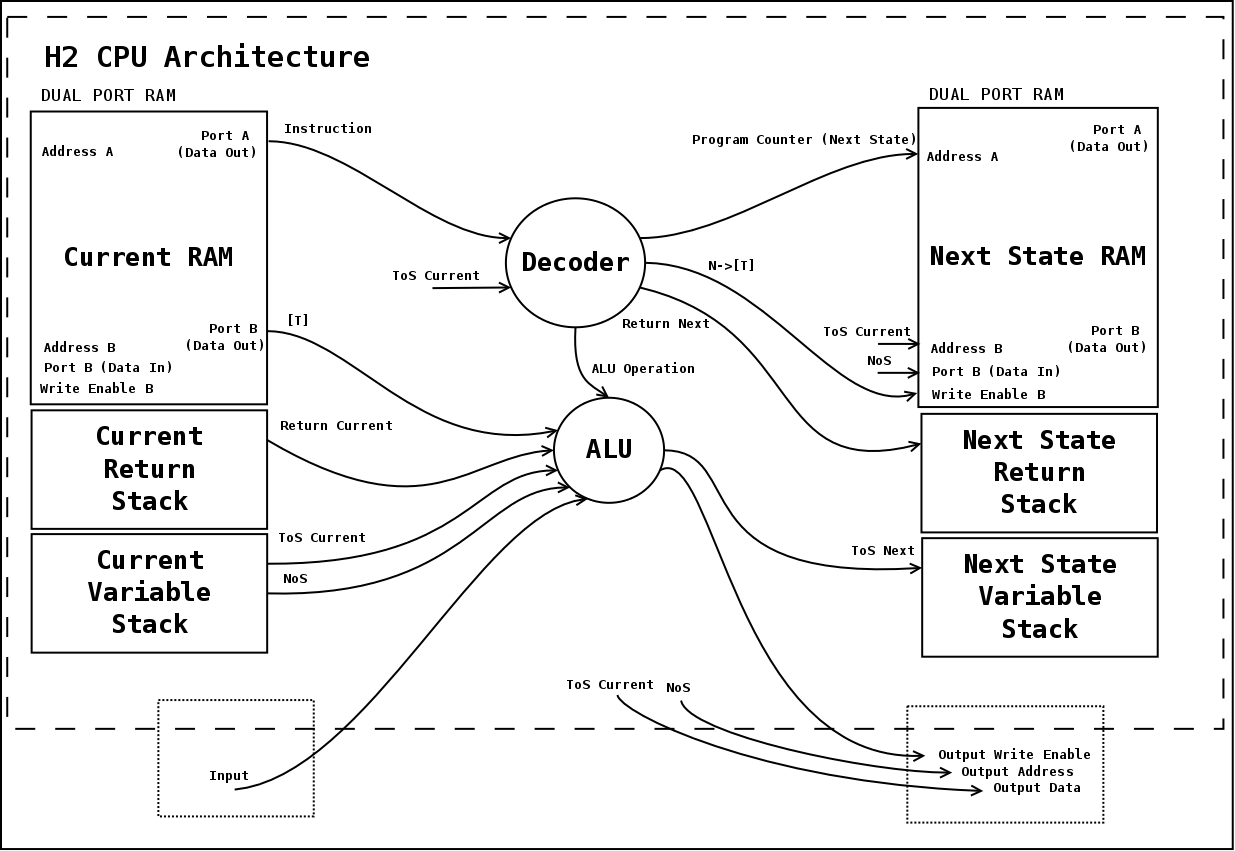
\includegraphics[width=1.1\textwidth]{pic/h2.png}
        \caption{The H2 CPU Core}
        \label{fig:H2 CPU Core}
      \end{figure}
      \FloatBarrier

      Most FORTH instructions can be executed in a single clock cycle, for example to add two numbers
      three separate instructions have to be run simultaneously for it to happen; a ALU T+N, N$\to$T and
      a data stack delta of $-1$.

      Jump indirection can be performed, however it would take multiple clock cycles to do so; First any
      calculations and fetching of data for the address have to be done which would take an indeterminate
      amount of time depending on what you want to do, then the data would have to be moved to the return
      stack (T$\to$R) and then after this R$\to$PC along with the relevant stack deltas. This takes a
      minimum of three cycles making it more expensive to do.

    \subsection{VGA}

    The VGA module acquired online at \cite{vgacore} provides an 80 column by 40 row text buffer with
    a resolution of 640 by 480. It is simple to interface with and required only minor modifications
    to get up and running.

    A picture of the output can be seen here with a test pattern loaded into the text buffer RAM:

      \begin{figure}[ht]
        \centering
        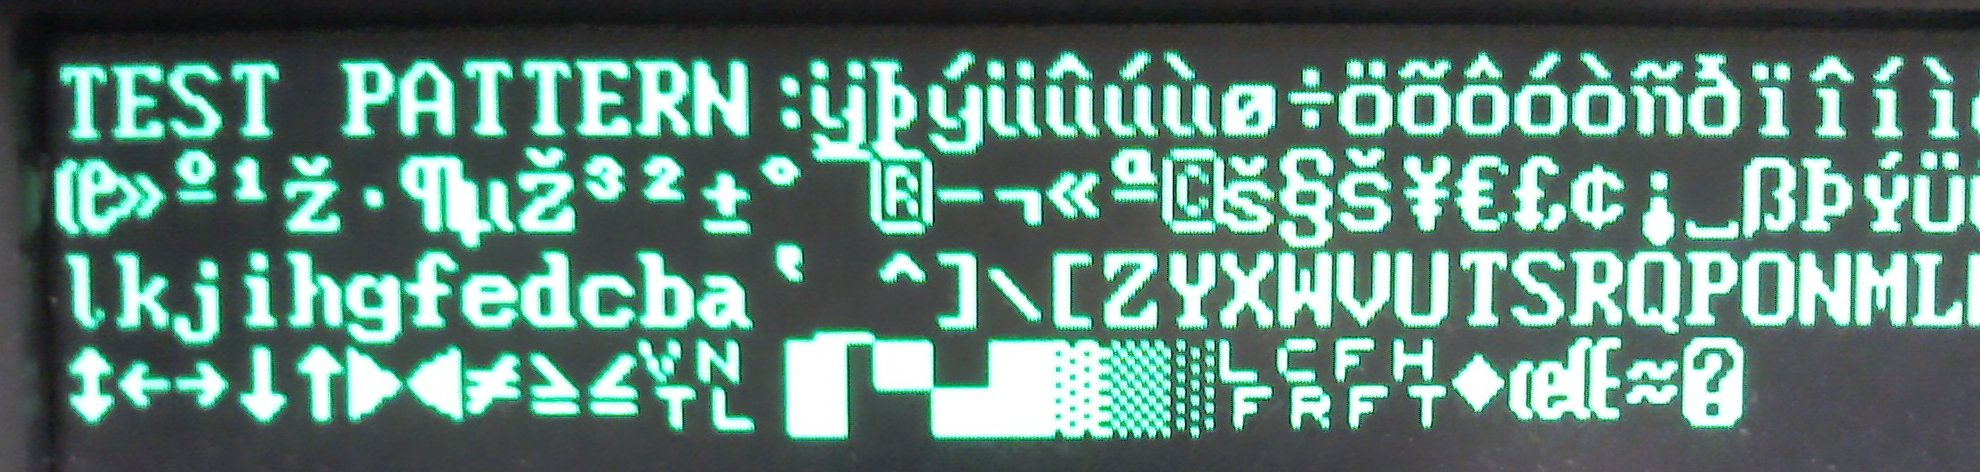
\includegraphics[width=0.8\textwidth]{pic/vga.png}
        \caption{VGA test pattern}
        \label{fig:VGA test pattern}
      \end{figure}
      \FloatBarrier

    To interface with this two BRAMs are initialized, one with the test pattern, the other with
    a font (the font BRAM actually acts as a ROM, but internally they are the same device). To
    use the unit there are only a few controls, a single control register (on/off, colour output,
    etcetera), two cursor positioning registers and the BRAM text buffer, simply write what you
    want to that buffer and it will be displayed on the screen.


    \subsection{UART}

      The UART is the primary method of talking to the device, it is customizable at
      compile time where the baud rate can be set. This module was acquired online
      and is in the references\cite{uartcore}. It is a standard UART core that is
      interfaced to the H2 in the top level. It is capable of both transmission and
      reception. I will want to rewrite this section in the future to bring it into
      line with exactly what I would like, it currently gives many warnings when
      synthesized, none of which cause any problems at the moment.

    \subsection{RAM and other inferred modules}

      Instead of using Xilinx specific components you can use VHDL to create code that
      fits a certain template, this template is picked up by the synthesizer and you  
      can then verify if this is what you intended. Using this instead of instantiating
      proprietary blocks and loading the RAM contents with proprietary tools is a much better
      way of doing things that allows me more flexibility in how I go about things.

      The VGA unit and the CPU both have their own RAM blocks, two for the former and
      one for the latter. They are initialized from an ASCII encoded binary format,
      which while not efficient is certainly easy to process with the given tools.

      For a given file describing the RAM, for example \textbf{"h2\_mem.vhd"}, 
      the initial contents will be described in a file called \textbf{"h2\_mem.binary"}.

      All the RAM used is dual port, this greatly simplifies the design. If I had to use single
      port RAM I would have to worry about moving data in and out of each module and the
      timing of the movements in much greater detail, it would also slow a lot of things down. For example
      the CPU would either have to adopt a Harvard architecture instead of a Von Neumann 
      or suffer a slow down.

    \subsection{Top level}

    The top level (\textbf{top\_level.vhd}) is an important piece of the project, it brings all of
    the modules together and handles input and output (this should be moved into a module
    of it's own). It also provides an interface between the outside world and the FPGA internals
    (ie. What the User Constraints File maps to).

    Stimulus is provided for simulation purposes by \textbf{test\_bench.vhd}, technically the
    highest up module, but only for simulation. 

    \subsection{Test benches and waveforms}

      Below is a waveform for a simple program along with said simple program further down:

      \begin{figure}[ht]
        \hspace*{-3.5cm}
        \centering
        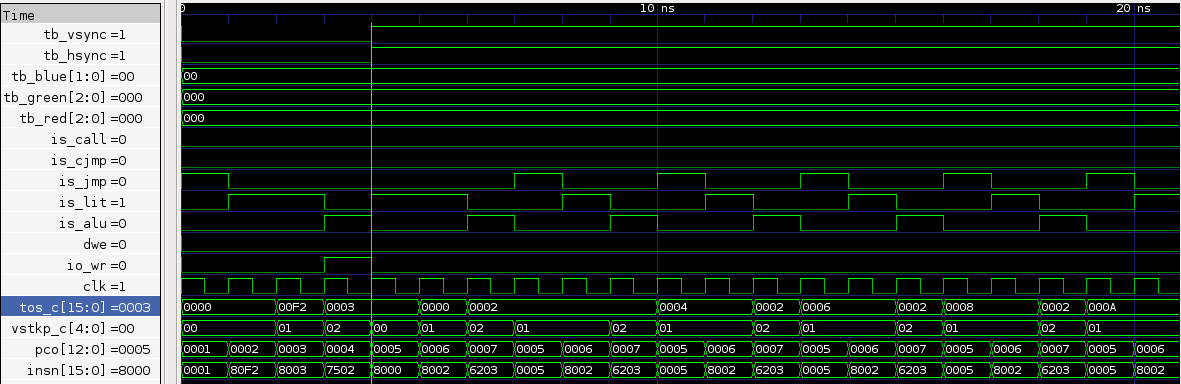
\includegraphics[width=1.6\textwidth]{pic/wav_adder.png}
        \caption{Adder waveform}
        \label{fig:Adder waveform}
      \end{figure}
      \FloatBarrier

      This program sets up the VGA control register then loops around adding two to the top
      of the stack.

\begin{verbatim}
242 constant o_vgaCtrlDefault 
3 constant o_vgaCtrl
: [SETUP]
    o_vgaCtrlDefault lit
    o_vgaCtrl lit 
    _output
;
start
  [SETUP]
  0 lit
  label main
      2 lit
      _+
  main jmp
stop 
\end{verbatim}

    Now given the waveform how can we show that this processor is running that code? It turns
    out that unless you want to do some more in depth debugging of a problem you do not really
    need to know what is going on in that many registers.

    The following registers suffice for most needs; \textbf{tos\_c, vstkp\_c, pco} and \emph{insn}.
    With these you can see what the current instruction being executed is each clock cycle as
    well as its result and effects on the variable stack pointer. (tos\_c is the top of the stack,
    vstkp\_c is the stack pointer, pco the address of the instruction to be executed and insn the
    instruction. 

    All this program does is set up the VGA control registers, push zero onto the stack and
    repeatedly add two to that number, we can see the VGA signals (\textbf{tb\_vsync} and \textbf{tb\_hsync}
    go high the clock cycle after the instruction "\_output" is executed in our code (Hex number
    7502). After this a zero then a two are pushed to the stack, then the two added to zero,
    accounting for the first long two which lasts for four clock cycles, after this is alternates
    between two and the current number that is to being added to. A simple test program which
    shows that this CPU works.

    We can also see what type of instructions are being execute with \textbf{is\_call, is\_cjmp,
    is\_lit} and \textbf{is\_alu}, each of which are pretty self explanatory given the instruction
    set encoding.

    Each time a new program is tested, it must be first checked with the test benches before going
    through the long process of synthesizing everything.

    This one shows the same code modified to subtract instead:

      \begin{figure}[ht]
        \hspace*{-3.5cm}
        \centering
        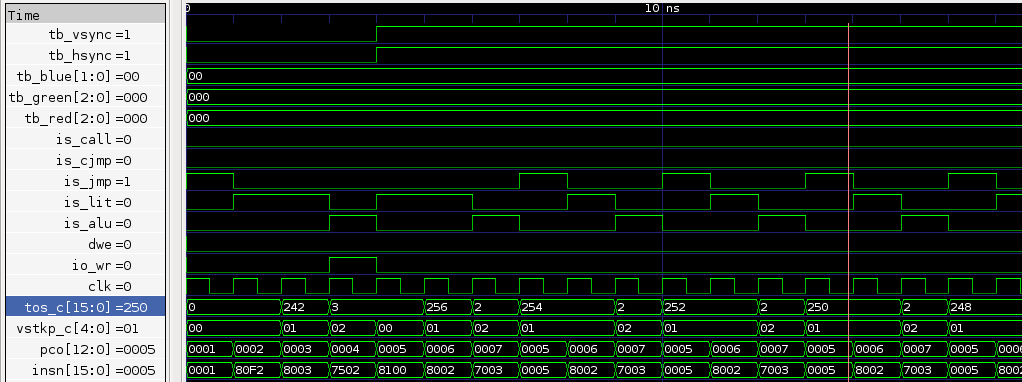
\includegraphics[width=1.6\textwidth]{pic/wav_sub.png}
        \caption{Adder waveform}
        \label{fig:Adder waveform}
      \end{figure}
      \FloatBarrier

    With the minor modifications:
\begin{verbatim}
start
  [SETUP]
  256 lit
  label main
      2 lit
      _-
  main jmp
stop 
\end{verbatim}

    And we can see it happily subtracting away!

    \subsection{Resource usage}

    To show you how little room the \emph{entire} design takes up (and hence how little the
    CPU takes up) here is a summary a report generated by Xilinx's tools.

\begin{verbatim}
Device utilization summary:
---------------------------

Selected Device : 6slx16csg324-3 


Slice Logic Utilization: 
 Number of Slice Registers:             303  out of  18224     1%  
 Number of Slice LUTs:                  814  out of   9112     8%  
    Number used as Logic:               780  out of   9112     8%  
    Number used as Memory:               34  out of   2176     1%  
       Number used as RAM:               32
       Number used as SRL:                2

Slice Logic Distribution: 
 Number of LUT Flip Flop pairs used:    879
   Number with an unused Flip Flop:     576  out of    879    65%  
   Number with an unused LUT:            65  out of    879     7%  
   Number of fully used LUT-FF pairs:   238  out of    879    27%  
   Number of unique control sets:        35

IO Utilization: 
 Number of IOs:                          46
 Number of bonded IOBs:                  46  out of    232    19%  

Specific Feature Utilization:
 Number of Block RAM/FIFO:               12  out of     32    37%  
    Number using Block RAM only:         12
 Number of BUFG/BUFGCTRLs:                2  out of     16    12%  
 Number of DSP48A1s:                      1  out of     32     3%  
\end{verbatim}

  Of note is how few LUTs and Slice Registers are used (8\% and 1\% respectively), and how
  many BRAMs are used (12), this shows that if we wanted to we could either fit more CPU cores
  onto the device or create our own really big devices to interface to it, the main limiting factor would be the BRAMs and
  the Slice LUTs used.

  The timing, that is the longest delay path, is subject to a more frequent and sensitive
  changes, if I am to issue one instruction per cycle the delay needs to be minimized to
  less than $10^{-9}$ seconds. As I am currently working on the project the maximum speed
  is roughly 97MHz, while I was demonstrating the project it was about 102MHz which is what
  we want, if I want to include my new changes I will either have to accept a slow down and
  work around it or minimize that delay, and the delay is easy to find as the tools tell you
  were it is.

  Bellow is a partial example of the delay estimate and route:

\begin{verbatim}
Timing Details:
---------------
All values displayed in nanoseconds (ns)

=========================================================================
Timing constraint: Default period analysis for Clock 'clk'
  Clock period: 10.293ns (frequency: 97.149MHz)
  Total number of paths / destination ports: 106202 / 825
-------------------------------------------------------------------------
Delay:               10.293ns (Levels of Logic = 19)
  Source:            mem_h2_instance/Mram_ram8 (RAM)
  Destination:       h2_instance/tos_c_15 (FF)
  Source Clock:      clk rising
  Destination Clock: clk rising

  Data Path: mem_h2_instance/Mram_ram8 to h2_instance/tos_c_15
                                Gate     Net
    Cell:in->out      fanout   Delay   Delay  Logical Name (Net Name)
    ----------------------------------------  ------------
     RAMB16BWER:CLKA->DOA0  113   1.850   2.016  mem_h2_instance/Mram_ram8 
                                                  (cpu_insn<14>)
     LUT3:I1->O            1   0.203   0.924  h2_instance/Mmux_aluop<1>11_1 
                                              (h2_instance/Mmux_aluop<1>11)
    ...                  ...     ...    ...           ...
\end{verbatim}

  This goes on longer giving you the entire route that the path takes, minimize
  this and you minimize the delay in your design.

  One fairly trivial optimization in the design which brought resource utilization
  down from 23\% of the slice utilization down to its current value was to properly
  use the distributed RAM construct, before the entire stack could be accessed all
  at once which was not necessary, nor possible by the current set up, only the
  next on stack is necessary to access, the top is held in its own separate register.

  \section{Problems}

    There were two main problems in this project, the build time for the hardware
    implementation and the multitude of problems faced when debugging the system,
    both of which slow the project down.

    \subsection{Build time}

    Some languages like C compile fairly quickly, others provide an interactive
    environment that you can test quickly like python. Any HDL however takes
    a fairly long time to simulate and a very long time to turn this design into
    a working 'bit file' to be uploaded to the integrated circuit. This acts as
    a friction and a drag on the development process as going from a simple change
    in a single line of code to the hardware can take upwards of fifteen minutes
    (on my computer). Simulation takes up less of that time, but it is still
    impractical to simulated even a second of real time. 

    There are a few ways
    to mitigate this, the best one is to be right the first time when you commit
    to hardware, although this can be difficult, I didn't have the time to create
    an adequate test bench to simulate incoming UART data for example, which made
    debugging the UART a slow process.

    The other simpler way is to use ever faster hardware, although that is an
    expensive option.

    \subsection{Debugging}

    Debugging can be awkward at best as there are many different places in which
    an error could occur and multiple errors could be conspiring to cause any
    given problem at hand. Why this is can be given by the list of places where
    a mistake could occur: The FORTH interpreter, the assembler, the assembly, the
    VHDL, the VHDL test-benches, the build system and finally the hardware implementation
    of what I have done could be different from the simulation. 

    The debugging process involves first pinning down where the error is as
    per usual, it is just made more unusually difficult by the fact that the error
    could be in so many different places. This is why an adequate test bench is
    a must.

    Eventually however as the system becomes more mature (for example I worked out
    many of the bugs in the assembler fairly quickly) the tools used also become
    more stable and reliable so you do not have to worry about them as much.

  \section{Documentation}

  In this section I will provide a terse (terse in the sense that this should
  be its own paper) description about the system.

    \subsection{FORTH interpreter}

    Instead of being a stand alone program with only one use I decided to create
    a full blown and reusable programming language in C, the reason for the extra
    complexity is because of its utility, I have used this program not only as an
    assembler but as part of the build process in ways that are not shown in the
    code (for example for converting between file formats).

    The interpreter can trace its lineage back to an entry to the IOCCC \footnote{
    The IOCCC is the International Obfuscated C Coding Competition, the entry can
    be found here: \url{http://www.ioccc.org/all/all.tar.bz2} in the folder '1992'
    for 'buzzard.2'.}. The interpreter is drastically different from the original,
    being a complete rewrite, although there are still similarities. 

    The program interprets threaded code \cite{threadedCode} for a stack machine,
    the C program does the initial heavy lifting allowing users to interpret commands
    but it is severely lacking in capabilities initially. The trick is to write most
    of the language \emph{in itself}. This maybe odd to people coming from a background
    in a 'normal' compiled and static language such as C/C++ or Java. You do not modify or extend
    the language itself but instead provide new functionality via libraries you have
    written in those languages.

    Initially the language does not even have basic elements such as the "if ... else ... then"
    statements or even loops, they are written in the language itself. FORTH, and my
    dialect of it, has the ability that its syntax can be changed arbitrarily. Lets say
    you want to make an interpreter for a different language, lets say lisp, you could
    do that and start executing lisp, while at the same time it would be a valid FORTH
    program as well.

    Of note is the fact that in FORTH terminology a 'Word' does not refer to a machine
    word but instead to a defined function, so when I refer to a 'Word' I mean function.

      \subsubsection{The C Program}

      The C program itself is design to be portable being written entirely in ANSI C \cite{ANSIC}, 
      I have had this program running on my phone, and plan with some minor adjustments
      to have this running on a few embedded systems as a testament to its portability.

      The C program is a threaded code interpreter and executes something which looks
      kind of like FORTH, although there are differences. It provides methods for
      extending the language, arithmetic and logic operations, conditional jumps,
      stack manipulations, writing to/from memory and input and output functions. It
      only supplies a basic set of primitives which are:

      \begin{itemize}
        \item \textbf{":"}: Read in a word and compile a header for it in the
        dictionary, switch to \emph{compile} mode.
        \item \textbf{"immediate"}: immediate is an \emph{immediate} word which
        makes the current word under going compilation \emph{immediate}.
        \item \textbf{"read"}: Read in a space delimited word, if it is in the
        dictionary and we are in compile mode, compile a pointer in the dictionary
        to the found word, else execute it, else if it is a number push it onto
        the variable stack, else there is an error.
        \item \textbf{"$\backslash$"}: Ignore input stream until end of line 
        (ie. A comment).
        \item \textbf{"exit"}: Return from a function call.
        \item \textbf{"br"}: Branch unconditionally to address held in address
        after this instruction.
        \item \textbf{"?br"}: Same as "br" except branch conditionally when
        the top of the stack is zero.
        \item \textbf{"+"}: Pop two numbers off the variable stack, add them
        and push the result.
        \item \textbf{"-"}: \ditto Subtract them \ditto 
        \item \textbf{"*"}: \ditto Multiply them \ditto
        \item \textbf{"\%"}: Pop two numbers off the variable stack, 
        and work out the remainder when the second item off is divided by
        the first, push the result.
        \item \textbf{"/"}: \ditto, divide the second item off by the first
        off, push the result.
        \item \textbf{"lshift"}: Logical shift left the next on stack by
        first on stack places. Push the result.
        \item \textbf{"rshift"}: \ldots same but with right shift.
        \item \textbf{"and"}: Pop two numbers, compute logical conjunction of them,
        push the result.
        \item \textbf{"or"}: \ldots same but with logical disjunction.
        \item \textbf{"xor"}: \ldots same but with exclusive disjunction.
        \item \textbf{"*~*"}: Bitwise inversion of top of stack.
        \item \textbf{"1+"}: Add one to top of stack.
        \item \textbf{"1-"}: Subtract one from top of stack.
        \item \textbf{"clear"}: Clear top of stack.
        \item \textbf{"0>"}: Test if top of stack is less than zero, push result.
        \item \textbf{"="}: Pop two numbers off variable stack, test for equality,
        push result.
        \item \textbf{"<"}: Pop two items off the variable, test if the first if
        greater than the second, push the result.
        \item \textbf{">"}: \ldots same but the inverse.
        \item \textbf{"@reg"}: Use top of stack as index into the array of
        registers, push what is in there on to the variable stack.
        \item \textbf{"@dic"}: Use top of stack as index into the dictionary,
        push what is in there on to the variable stack.
        \item \textbf{"@var"}: Same but with the variable stack itself.
        \item \textbf{"@ret"}: Same but with the return stack.
        \item \textbf{"@str"}: \ldots with string storage.
        \item \textbf{"!reg"}: Store next on stack into the address pointed
        to by the first on the stack into the register file.
        \item \textbf{"!dic"}: \ldots into the dictionary.
        \item \textbf{"!var"}: \ldots into the variable stack.
        \item \textbf{"!ret"}: \ldots into the return stack.
        \item \textbf{"!str"}: \ldots into string storage.
        \item \textbf{"key"}: Push one changed from the input to the
        variable stack.
        \item \textbf{"emit"}: Pop one character from the variable stack,
        and output it.
        \item \textbf{"dup"}: Duplicate top off the variable stack.
        \item \textbf{"drop"}: Drop top of variable stack.
        \item \textbf{"swap"}: Swap top two items of variable stack.
        \item \textbf{"over"}: Duplicate the second item on the variable stack. 
        \item \textbf{">r"}: Move an item from the top of the variable
        stack to the return stack.
        \item \textbf{"r>"}: \ldots the other way around.
        \item \textbf{"tail"}: Word used for recursion, call this primitive
        then the word you want to use recursively.
        \item \textbf{"'"}: Push the next compiled word onto the stack at
        run time.
        \item \textbf{","}: Advance dictionary pointer, pop the top of stack
        and write in into the dictionary.
        \item \textbf{"printnum"}: Use the top of the stack as an index into
        a string in string storage, treat this as a number and print it.
        \item \textbf{"get\_word"}: Use the top of the stack as an index into
        string storage, store a space delimited string there.
        \item \textbf{"strlen"}: Pop the top of the stack and use it as an index
        into string storage, compute the string length and push the result.
        \item \textbf{"isnumber"}: Pop the top of the stack and use it as an index
        into string storage, test if the string is a number or not and push the
        result.
        \item \textbf{"strnequ"}: Pop two numbers off the stack and use both
        as indices into string storage, compute whether or not the strings are
        equal; zero is pushed if they are, one if they are not, two if the strings
        are too long ('too long' is determined in the source).
        \item \textbf{"\_find"}: Find a word in the dictionary if it
        exists and push a pointer to the beginning of the word header if
        it does.
        \item \textbf{"halt"}: Halt the system.
        \item \textbf{"kernel"}: Use the top of the stack to perform an
        external call. All calls have access to all the memory.
      \end{itemize}

      Also defined but not present here are three 'hidden' words, that is
      words with no name which are:

      \begin{itemize}
        \item \textbf{"Push integer"}: Pushes the next instruction onto the
        data stack, advances program counter over instruction.
        \item \textbf{"Compile"}: Compile a pointer to the execution token
        'Run' of a word.
        \item \textbf{"Run"}: Run a word, saving the return address onto the
        return stack.
      \end{itemize}

      The word ";" has not been defined here, it instead defined later like
      more of the standard words such as "rot" (rotate first three stack
      items). 

      The best documentation is the code itself, it is not too long, but
      I will give a quick overview of what happens.

      The memory is initialized, a function that is created that calls
      'read' then calls itself (read also handles this so the return stack does
      not blow up), this forms the basic command interpreter.

      Before this is run a list of symbols is read in which forms the
      names of the primitives in the dictionary. Then the function it has created
      is executed.

      There are two states the interpreter can be in, compile or command
      mode, in compile mode (which is what we start out in) if a word is
      found a pointer to that word is compiled into the dictionary, in
      command mode it is executed instead. There is a certain class of
      words that are always executed and they are called \emph{immediate}
      words.

      Each word compiling has the following structure:

      \begin{center}
        \begin{tabular}{l | c | c | c | r }
          \hline
          prev & str & \textbf{compile} & run & data field \ldots \\
          \hline
        \end{tabular}
      \end{center}

      Each immediate word has this structure:
      
      \begin{center}
        \begin{tabular}{l | c | c | r }
          \hline
          prev & str & \textbf{run} & data field \ldots \\
          \hline
        \end{tabular}
      \end{center}

      Where "prev" is a pointer to the previous word, "str" a pointer to the words
      name, "compile" is the instruction compile if present and "run" is the instruction
      "run". The text in bold is what is run when the word is found by "read", what makes
      the difference between an immediate and a compiling word is what is pointed to.

      The data field is of a variable length and in a normal word consists entirely or
      either pointers to other words execution field (run), numbers
      to push onto the stack or places to jump to (after either "push" or one of the
      branch instructions respectively).

      The dictionary consists of a linked list of words, and each words data field
      consists of pointers to other words making for very compact code.

      There are two stacks, a variable stack where computations are generally performed
      and a return stack for return from functions and as temporary storage. The other
      chunks of memory include a register file which contains pointers to the next
      word and instruction to execute, a pointer to the previously defined word, stack
      pointers, a pointer into the next available dictionary address as well as some
      information about the virtual machine itself. Then there is the dictionary which
      contains all the defined words as well as being used as a general storage facility.
      Finally there is a string storage space, used to store the names of words and
      other strings.

      While this description is lacking, I do have a limited space I have to write about
      each of the components so for brevities sake I will have to refer you to the
      actual code itself.
       
      \subsubsection{Basic commands and ideas}

      After the basic word list has been defined we then define more FORTH words and
      bring the interpreter/compile into a working state, loops and conditional
      statements as well as words for debugging and file operations are introduced
      here. After this the constants and system necessary for the assembler are made,
      because the assembler is still executing in the FORTH environment you can still
      call any previously defined word there.

      To interpreter is currently set up to read a start-up file, \emph{start.fs}
      which then reads the assembly file \emph{h2.fs} and outputs that to the right
      directory.

      To run the interpreter only, you would need to edit the file \emph{start.fs}
      to not run \emph{h2.fs}, which is a trivial change at the end of the file,
      just delete the lines:

      \begin{verbatim}
foutput ../vhdl/mem_h2.binary
finput h2.fs
      \end{verbatim}     
       
      You can then run the interpreter (./forth) and type 'words' to get a list of
      defined commands.

      To get a better understanding of how this interpreter works consult the
      IOCCC submission 'buzzard.2' from 1992 \cite{ioccc}

      A more up to date, better documented and more standalone version also
      written by myself is available at: \url{https://github.com/howerj/c-forth}.
      This is the main branch from which this I used in this project is
      based.

    \subsection{H2 CPU}

    The H2 CPU has already been described, it is not too big and the VHDL in the
    appendix can be read and understood by someone with minimal understanding of
    the language.

    I will instead document the assembly used.

      \subsubsection{Assembly}

    The assembler is written in a few hundred lines of FORTH, it is mostly
    several constants and a few helping functions specific to the H2 processor
    near the end of the file \textbf{start.fs}.

    Bellow is a very simple test program:

\begin{verbatim}
242 constant o_vgaCtrlDefault \ 11110010, VGA control register set to this.

\ Outputs
0 constant o_7seg
1 constant o_ledS
2 constant o_vgaCursor
3 constant o_vgaCtrl
4 constant o_vgaTxtAddr
5 constant o_vgaTxtDin
6 constant o_vgaWrite
7 constant o_uartWrite
8 constant o_uartStbWrite
9 constant o_uartAckDout

\ Inputs
0 constant i_buttons
1 constant i_switches
2 constant i_vgaTxtDout
3 constant i_uartRead
4 constant i_uartAckWrite
5 constant i_uartStbDout

\ ============================
\ Word definitions.
\ ============================

: [SETUP]
    o_vgaCtrlDefault lit
    o_vgaCtrl lit 
    _output
;

: [LED]
    o_ledS lit _output
;

: [SWITCH]
    i_switches lit _input
;


\ ============================
\ Begin program loop.
\ ============================
start
    [SETUP]
    label main
        [SWITCH]
        [LED]
    main jmp
stop
\end{verbatim}

    The actual program that is running on the FPGA begins at the word \emph{start}
    and ends quite naturally at the word \emph{stop}. It simply sets up the VGA
    to display the test pattern and after it has done that it loops around
    constantly read the input switches and displaying them on the output LEDs. It
    was the first program run on the FPGA, one which is just a simple test that
    everything is working.

    As you can see you can call functions defined in the FORTH interpreter. In the
    example several words are called: \emph{'constant',':','$\backslash$'} and \emph{';'}. We can
    define new words in the assembler to help us out with ':', simple macros in
    this case \emph{[SETUP],[LED]} and \emph{[SWITCH]} that expand into the machine
    instructions they contain.

    The program is only written out when \emph{'stop'} is reached so messages
    about the program assembly progress can be written out to the standard terminal
    output.

    Let us look at how an instruction works and how it is assembled. We can start
    with the simple addition instruction called \emph{\_+} in the assembler to
    avoid confusion with the FORTH instruction by a similar name, +. 

    The definition of this is as follows:    

\begin{verbatim}
: _+ alu[ T+N d-1 or ]alu ;
\end{verbatim}

    Analysing this word by word:

    \begin{itemize}
      \item \textbf{':'}: Begin the compilation of a new word in the dictionary.
      \item \textbf{'\_+'}: The name of the new word.
      \item \textbf{'alu['}: This is simply some syntactic sugar, it does not
      do anything but looks better with a corresponding ']alu'.
      \item \textbf{'T+N'}: This pushes the value of whatever the ALU instruction
      is to the variable stack.
      \item \textbf{'d-1'}: This pushes the value of a variable stack decrement
      for out CPU.
      \item \textbf{'or'}: As a stack decrement and an ALU instruction (amongst
      other things) can occur within the same instruction we merge these into
      one.
      \item \textbf{']alu'}: This merges the instruction we want with a header
      ('011' in the high bits of the instruction) that signifies that this is
      an ALU operation and not for example, a conditional jump. It then writes
      this out into a memory model of our CPU and increments a pointer to the
      next available memory location in it.
      \item \textbf{';'}: This of course ends the current word definition.
    \end{itemize}

    This allows us to create an assembler along with definitions along with labels
    which allow us to name a memory location for out program to jump to.

   \section{Future plans}
    \label{sec:futurePlans}

    I intend to keep working on this project after I have finished university, it offers the
    potential to provide a nearly complete laboratory work bench for home use as I will talk
    about.

    There are some general improvements that could be made; making the code more uniform
    through out, adding variable stack sizes and word sizes, improving the instruction set,
    much more thorough testing (and proofs there of).

    The potential improvements here are outside the scope of the project, they were never
    intended to be included in it as I would not have had time to do so, however when I
    started the project I did have these as an eventual end goal. The platform has a lot of
    potential.

    This section is fairly big despite not actually documenting the project due to the fact
    that it in part \emph{justifies} the project, this section actually more or less provides
    the reasoning for me starting the project.

    \subsection{Hardware}

      The hardware section is the one that offers the most potential when it comes to
      what can be improved with the device, although it is the section that will move
      most slowly as HDLs can be difficult to debug, more so than normal programs.

      \subsubsection{Different platforms}
      One of the goals of this project was portable of code and not just to different
      Xilinx devices either. I would like to port this system to cheaper hardware
      such as the "Papilio One". \cite{papilio} This system while less
      functional costs a fraction of the Nexys 3. While the project would be more
      constrained, it should still be able to fit on the device with ease.

      I would like to get my code running on as many platforms as possible, while it
      \emph{should} be portable you can never truly find out until you have tested
      it on the real thing.

      \subsubsection{More generic code}

        If possible I would make my code as generic as I could. What I mean by this
        is being able to specify most of the parameters such as instruction size
        width and RAM size just by editing a few variables. Some of this might be
        easier than other parts to do so. An example of a difficult-to-make-generic piece of code
        would be in the H2 CPU core:

        \lstset{language=VHDL,caption={Stack Depth Instruction},label=stackDepthVHDL} 
        
\begin{lstlisting}
when "01110" =>  tos_n   <=  vstkp_c & "000000" & rstkp_c; 
\end{lstlisting}

        This instruction takes two stack pointers and puts them on to the stack so
        you can analyse them. However if I wanted to increase the size of the
        stack the pointers would also increase in size, taking up more room and
        rendering this instruction incorrect.

      \subsubsection{PS/2 or USB keyboard}

      A PS/2 Keyboard could be added to the board, the Nexys 3 provides a USB
      to PS/2 interface, this could be used to interact with the system instead
      of the computer.

      \subsubsection{Signal Generator}

      A signal generator should be fairly easy to design, at least internally, the
      main problem would be designing the external analogue components to work from
      ~1Hz to 100MHz (or a fraction thereof).

      The VHDL would consist of a block RAM holding the data, for example a sine wave
      or another arbitrary signal, a counter, a pointer into the memory and a few
      registers to control the device. As the RAM being used is dual port, it is
      possible to run two signals from the same RAM at a sacrifice of precision.

      This would be output in parallel over some of the boards standard I/O pins
      to a digital to analogue converter.

      \subsubsection{Data logger}

      By hooking up an external Analogue to Digital Converter (ADC) and a few other
      circuits it would be possible to have a fairly high speed data logger where
      plotting could be handled in real time on a normal computer (depending on how
      fast I manage to sample things).

      This would be the most difficult to add section and it would also be the one
      that would provide most in the way of utility.

      \subsubsection{Logic Analyser}

      With very minimal additions a logic analyser running at the speed of the device
      ($\frac{1 Sample}{Clock Cycle}$) should be attainable, the unit does not have
      to be directly controlled by the CPU core, perhaps only by setting a few registers
      to tell it how fast to sample and how much, when to begin and end and where to
      send the data.

      I can see the main problems being in where to store the data and how to get it
      off the board, I would need a faster method of communications than the UART
      unless I only intend to capture roughly 16 Kilobytes of data at a time.

      The external hardware would be quite simple, just a way to buffer and electrically
      isolate the signal from the input pins of the device.

      Instead of displaying the data on the device, it should be done instead on a
      normal desktop, at least initially.

      \subsubsection{Multiple cores}

      Due to the tiny amount of resources that are taken up by the CPU it should be
      possible to have more than on CPU core running on the platform at the same
      time, perhaps a dedicated CPU for each peripheral with one master? It would
      be a relatively easy way of increasing the power of the system.

      This is however not a priority, first increasing functionality of the base
      system by adding the aforementioned peripherals would be of greater initial
      utility, then adding more cores would be considered.

      \subsubsection{Miscellaneous}
      
      The addition of timers, the reintroduction of the multiplier and adding 
      interrupts to the new CPU core would all improve the system as a whole.

      There are also several different types of memory on the Nexys 3 board
      which could be interfaced with which would allow me to overcome the
      limitations of the H2's memory restrictions, instructions could be swapped
      in and out.

    \subsection{Firmware}

    The firmware is what could receive the most drastic improvement, getting a small
    interpreter up and running on this device is a priority. This would allow it
    to be used as a standalone system, one which I believe would be fairly useful
    to multiple people. 

    This is where the real complexity in the device would lay, eventually.

    \subsection{Build system}

    I would like to replace most of the build system with my FORTH interpreter as I
    think it would be a good show case of the language I designed, it would need
    a way for it to deal with multiple files at the same time which it currently does
    not, along with a few trivial improvements, but once that has been done I could
    use it as a replacement for all the miscellaneous shell scripts and makefiles
    that I have.

  \section{Conclusion}

    In this final section I will summarize my project achievements as well as describe
    what I would or could have done differently if I were to do this project again.

    \subsection{Project achievements}

    From the section of "Future Plans" you can see that I have some grand ideas when
    it comes to what will happen with this project next and given that, I would of course
    like to achieve even more than I did regardless of how much I actually got done.

    I did however achieve nearly all of my objectives when it came to this project and
    met one of the optional ones which I believe makes this an overall win.

    I would have liked to have tried even more different instructions out with the processor and
    tried to optimize it for my needs, my primary concern was getting it working but
    there are few instructions that could be merged into one and a few others that can
    be replaced if for example a few of the bits were used for signed addition, below
    is an example of what I mean.

    As I did not end up using the full range of the CPUs ALU bits (there are 24 instructions
    leaving space for further instructions, all of the bits are used, just not the full range)
    I could add a simple instruction that would implement signed addition. A prefix of "111"
    would signify that the remaining two bits should be added to the current top of the stack
    allowing deltas of $+1,0,-1,-2$, as adding zero is not entirely useful this could used for
    something else making the most efficient use of space possible.

    \begin{center}
      \begin{tabular}{l | c | c | c | r }
        \hline
        1 & 1 & 1 & Sign & Number \\
        \hline
      \end{tabular}
    \end{center}

    While this may not be the best method of doing things, I would have at least liked to
    have tested this out and compared the results.

    I believe that my project has gone well however and has achieved its primary goals.

    \subsection{What I would have done differently}

    If I could do this project again I would have tried to make even better test benches
    to automate even more than I did. It is possible to automatically test all
    the major instructions instead of manually looking at waveforms. The problem laid in
    the fast paced changes that I implemented, there was no use in creating tests for the
    system if it was to change a few hours or minutes later as I was experimenting on 
    everything.

    As I have said, I would liked to have played more around with the CPU and that has
    already been addressed.

    One more things I should have done is integrate more of other people's cores into
    my system, it increases functionality greatly and is not too difficult given one
    conditional is satisfied; \emph{if you can find a good enough core}. Otherwise you
    can spend a good deal of time debugging your code and how you interface to things
    until you realize it is not your project that is the problem but some one else's
    code. More cores can be found at opencores.org\cite{opencore}.

    I would have also worked on improving the FORTH interpreter, not the C program
    section but the actual assembler itself, it is certain powerful enough for the
    development of test programs and a bootloader but it's limitation become apparent
    after more usage.

    \subsection{Final words}

    While giving the poster presentation a number of lecturers expressed an interest
    in my project and its future, specifically the capability for it to act as a
    signal generator or be part of some kind of DIY electronics laboratory, I am as well,
    so rest assured that this project will continue and check in in perhaps a year or 
    two to monitor the progress made.

    I am pleased with how this project went and I think I have managed to accomplish
    quite a lot; I would like to thank Marc Eberhard, my project supervisor and Kate
    Sugden, my course director for their help. Also I would like to thank all those
    people whose code has been incorporated in one form or another into this project.

  \section{References}

    \bibliographystyle{plain}              % Use plain style
    \begin{thebibliography}{1}              % Simple bibliography with widest label of 1
    \bibitem{nexysDigilent} $Nexys^{TM}$3: \emph{A FPGA Spartan-6 development board}, \url{http://www.digilentinc.com/Products/Detail.cfm?NavPath=2,400,897\&Prod=NEXYS3}, (2013)
    \bibitem{xilinxDataSheet} XC6LX16 Family Overview: \emph{Spartan-6 Family Overview}, \url{http://www.xilinx.com/support/documentation/data_sheets/ds160.pdf}, (2011)
    \bibitem{CLB1} Mark Oskin : \emph{Advanced Digital Design: CSE 467 - Winter 2003}, \url{http://www.cs.washington.edu/education/courses/cse467/03wi/FPGA.pdf}, (2003)
    \bibitem{j1core} James Bowman, Willow Garage: \emph{J1: A small Forth CPU for FPGAs},  EuroForth 2010, \url{http://www.excamera.com/files/j1.pdf} (2010)
    \bibitem{newwave} Philip J. Koopman, Jr: \emph{Stack Computers: the new wave}, \url{http://www.ece.cmu.edu/~koopman/stack_computers/sec6_2.html}, chapter 6, section 2 (1989)
    \bibitem{threadedCode} Anton Ertl: \emph{Threaded Code}, \url{http://www.complang.tuwien.ac.at/forth/threaded-code.html}, (2013)
    \bibitem{vgacore} Javier Valcarce: \emph{VHDL Macro: VGA80x40}, VHDL Monochrome VGA display adapter ,\url{http://www.javiervalcarce.eu/wiki/VHDL_Macro:_VGA80x40} (2009)
    \bibitem{uartcore} Peter Bennett: \emph{RS232 UART (VHDL)}, A UART core, \url{http://bytebash.com/2011/10/rs232-uart-vhdl/} (2012)
    \bibitem{ANSIC} ANSI/ISO C: \emph{ISO C Standards Website for the C Standard}, \url{http://www.open-std.org/jtc1/sc22/wg14/www/standards} (1990)
    \bibitem{papilio} Papilio One: \emph{A Cheap FPGA development board}, \url{http://papilio.cc/},2013
    \bibitem{ioccc} IOCCC winner Buzzard: \emph{An obfuscated FORTH interpreter}, \url{http://www.ioccc.org/1992/buzzard.2.design}, (1992)

    \bibitem{opencore} Opencores: \emph{Open source HDL cores and code}, \url{http://opencores.org/projects} (2013)

    \end{thebibliography}



  \section{Appendix}

  \subsection{H2.VHD}
  I am going to include the code for the H2 code as this forms the core of the project, for
  the other files go to the Github account. For instructions on how to run this consult the
  file "README.md" in the repository. The contents of this repository should be made available
  as a separate folder along with this report.

  Also of note, you can look through the repository to find out how the work flow went, it
  does not include the beginning of the project, only about a month before the end, it does
  show how certain things progressed however.

  \lstinputlisting[language=VHDL]{../../vhdl/h2.vhd}

  \subsection{Original specification}

      Here is the original specification for the project which can be found in the repository
  in full also under the name "spec.pdf".

      \subsubsection{FPGA: Main plan.}

      As I have said, this would be my main plan, to use an FPGA to make my own
      computing system, this is not infeasible and has done before, my own design
      will be unique and customized to the task I want it to do.

          While it will not be useful as a general purpose computer, it could be used
      for pedagogical purposes, both for me and for other people as well.

          The hardware would be very simple, and at minimum would be a Nexys 3
      development board, with a serial connector interface. The FGPA contained in
      the device is a Xilinx Spartan-6 XC6SLX16 which is enough to fit my project
      on along with enough internal RAM to run its program.

      \noindent \textbf{Deliverables}

      The following are a list of the projects deliverables.

        \begin{itemize}
        \item CPU and Waveforms.
        \item Cross assembler.
        \item Serial Interface.
        \item FORTH language interpreter.
        \item (Optional): Keyboard Interface.
        \item (Optional): VGA Interface.
      \end{itemize}
      The last two being entirely optional, it all depends on how feasible it is to make
      the last two.

      \noindent \textbf{Languages to use}

      The following is the languages I wish to use, for a variety of tasks, from hardware
      description, to automation.

      \begin{itemize}
          \item  VHDL: Hardware description of CPU core and peripherals.
          \item  VHDL: Test Benches for hardware.
          \item  Python: Cross Assembler.
          \item  Assembly: Used to write the FORTH interpreter in.
          \item  FORTH: Ultimate goal of the project, a FORTH language interpreter.
      \end{itemize}

      Other miscellaneous languages used will be \LaTeX for writing up the report, GNU
      Make files for the build system, and Bash shell scripts for automating simple
      tasks. The Git version control system will be used to keep track of the latest
      build and documentation.

      \noindent \textbf{Industry and other standards}

      As I have said I will be linking to other standards, which I will use in my project,
      some of which will be part of optional modules such as the Keyboard and VGA
      (video) output.

      \begin{itemize}
          \item  J1 Processor Core: Described in a paper 4 and written in Verilog, this will
          be rewritten in VHDL and modified.
          \item  Serial Port: This is a very well known standard, and will form the primary
          interface between the outside world and my CPU core.
          \item  VGA standard : A well known Video standard (optional)
          \item  PS/2 Keyboard (Optional)
      \end{itemize}

      \noindent \textbf{Software to use}

      I already have the software and build environment set up and ready to be used,
      I will have to adapt some Makefiles for my purpose, but apart from this, the
      software environment I will be working on is ready. The project will be developed
      in a Linux environment (Debian 6.0), using Xilinx Webpack (Latest version),
      and Digilents drivers. Other software that is relevant to the project is Git, for
      versioning, GNU make, and finally, GHDL for simulation purposes only.

      \noindent \textbf{J1 Processor}

      Instead of specify my own instruction set, I am going to use on that is already
      specified for me, as my device does not have to fit into such a small space, I
      can utilize much more of the chip if I want to, the original processor had to fit
      inside a cameras FPGA that had many other tasks to do.

          I could experiment with optimizing the core for my specific needs, for example
      , I could decide if I want to use unsigned or signed arithmetic, I could also
      add more operations to the core (one bit is unused in the instruction set). I
      am refraining to say as to what I may add, I would like to see would are the
      bottlenecks in my design before I start to customize the core. A big boost would
      probably be having a general purpose multiply instruction, however I may be
      able to get away with a left shift for multiplication (by 2n only), and division
      by 2n as well (right shift).

          Depending on what I want to do, I could add instructions for cyclic shifts, or
      even more complicated things instructions tailored to my task. This is optional.

      \noindent \textbf{Error handling and multitasking (Optional)}.

      I would like to create a robust system, and I would like to do that on many
      levels, testing as much as possible and eliminating sources of error, in that
      vein, there could be certain systems in place for checking whether certain things
      make sense. Bounds checking could be enforced at the hardware level if needs
      be, making sure certain instructions can not be executing if they operate on
      data in off limits areas.

          Another possibility is to aid multitasking, either with multiple cores, or with
      banks of registers that can be switch to and from in a few instruction cycles.
      Both of theses tasks would be entirely optional.

        Again, the J1 Processor can be found here \url{http://www.excamera.com/sphinx/fpga-j1.html} 
        and here \url{http://www.excamera.com/files/j1.pdf}.

\end 	{document}
